\documentclass[12pt]{article}
\usepackage[utf8]{inputenc}
\usepackage[T2A]{fontenc}
\usepackage[english,russian]{babel}
\usepackage{amssymb,amsmath}
\usepackage{graphicx}
\usepackage[margin=2cm]{geometry}

\renewcommand{\vec}[1]{\boldsymbol{\mathbf{#1}}}
\newcommand{\tr}{\mathsf{T}}

\author{Цыбулин Иван}
\title{Линейные многошаговые методы \\ \vspace{2 mm} {\large Условия порядка. Устойчивость}}
\date{}

\begin{document}
	
\maketitle

\textbf{К2}. \emph{Для решения жесткой задачи коши из $n$ обыкновенных дифференциальных уравнений
\[
\vec y'(t) = \vec G(y, \vec y(t)), \quad \vec y(0) = \vec y^0,\quad t \in [0, T]
\]
предлагается использовать следующий линейный многошаговый метод
\begin{align*}
&a_2 \vec u_{n+1} + a_1 \vec u_n + a_0 \vec u_{n-1} = \tau \Big(
b_2 \vec G(t_{n+1}, \vec u_{n+1})+
b_1 \vec G(t_{n}, \vec u_{n})+
b_0 \vec G(t_{n-1}, \vec u_{n-1})
\Big),\\
&\qquad\vec u_0 = \vec y^0,\quad\vec u_1 = \vec y^1,\\
&\qquad a_2 = \frac{5}{6}, \;
a_1 = -\frac{2}{3}, \;
a_0 = -\frac{1}{6}, \qquad
b_2 = \frac{1}{3}, \;
b_1 = \frac{2}{3}, \;
b_0 = 0
\end{align*}
\begin{itemize}
	\item[а)] Указать порядок аппроксимации для разностного уравнения.
%	\item[б)] Исследовать разностную задачу на устойчивость по начальным данным для тестового уравнения $y' = \lambda y(t), \lambda \in \mathbb{C}$.
	\item[б)] Исследовать метод на $A$-устойчивость.
	\item[в)] Исследовать метод на $L$-устойчивость.
\end{itemize}
}

а) Условия порядка для линейного многошагового метода:
\begin{itemize}
\item Необходимое условие: $a_2 + a_1 + a_0 = 0$. Если его нарушить, метод не будет аппроксимировать никакую задачу.
\item Условие первого порядка и выше: $a_2 - a_0 = b_2 + b_1 + b_0$
\item Условие второго порядка и выше: $\frac{1}{2}(a_2 + a_0) = b_2 - b_0$
\item Условие третьего порядка и выше: $\frac{1}{6}(a_2 - a_0) = \frac{1}{2}(b_2 + b_0)$
\item Условие четвертого порядка и выше: $\frac{1}{24}(a_2 + a_0) = \frac{1}{6}(b_2 - b_0)$
\end{itemize}
Условие четвертого порядка противоречит условию второго, и для двухшагового метода выполняться не может. Иными словами, двухшаговый метод может иметь порядок не выше третьего.

В нашем случае выполнены необходимое условие $\frac{5}{6} - \frac{2}{3} - \frac{1}{6} = 0$, 
условия первого порядка $\frac{5}{6} - \left(-\frac{1}{6}\right) = 1 = \frac{1}{3} + \frac{2}{3} + 0$, условие второго порядка $\frac{1}{2}\left(\frac{5}{6} - \frac{1}{6}\right) = \frac{1}{3} = \frac{1}{3} - 0$ и условие третьего порядка $\frac{1}{6}\left(\frac{5}{6} + \frac{1}{6}\right) = \frac{1}{6} = \frac{1}{2}\left(\frac{1}{3} + 0\right)$. Следовательно, метод имеет третий порядок аппроксимации.

%б) Рассмотрим тестовое уравнение $y' = \lambda y, \quad \lambda \in \mathbb{C}$. Пусть $z = \tau \lambda$.
%\[
%a_2 u_{n+1} + a_1 u_{n} + a_0 u_{n-1} = z (b_2 u_{n+1} + b_1 u_{n} + b_0) u_{n-1}.
%\]
%Общее решение этого разностного уравнения имеет вид
%\[
%u_n = C_1 q_1(z)^n + C_2 q_2(z)^n,
%\]
%где $q_{1,2}(z)$ --- корни характеристического многочлена
%\[
%(a_2 - z b_2) q^2 + (a_1 - z b_1) q + (a_0 - z b_0) = 0.
%\]
%Для нашей задачи характеристический многочлен имеет вид
%\[
%(5 - 2z) q^2 - 4(1 + z) q - 1 = 0,
%\]
%а его корни
%\[
%q_{1,2} = \frac{2(1 + z) \pm \sqrt{4(1+z)^2 + (5-2z)}}{5 - 2z} = 
%\frac{2 + 2z \pm \sqrt{9 + 6z + 4z^2}}{5 - 2z}.
%\]
%Разложим $q_{1,2}(z)$ в окрестности $z = 0$ (это соответствует окрестности $\tau = 0$).
%\begin{multline*}
%q_1(z) = \frac{2 + 2z + \sqrt{9 + 6z + O(z^2)}}{5 - 2z} = 
%\frac{2 + 2z + 3\sqrt{1 + \frac{6z}{9} + O(z^2)}}{5 - 2z} = \\ =
%\frac{2 + 2z + 3(1 + \frac{3z}{9} + O(z^2))}{5 - 2z} = 
%\frac{5 + 3z + O(z^2)}{5 - 2z} = 
%\frac{1 + \frac{3}{5}z + O(z^2)}{1 - \frac{2z}{5}} = \\ =
%1 + z + O(z^2)
%\end{multline*}
%\begin{multline*}
%q_2(z) = \frac{2 + 2z - \sqrt{9 + 6z + O(z^2)}}{5 - 2z} = 
%\frac{2 + 2z - 3\sqrt{1 + \frac{6z}{9} + O(z^2)}}{5 - 2z} = \\ =
%\frac{2 + 2z - 3(1 + \frac{3z}{9} + O(z^2))}{5 - 2z} = 
%\frac{-1 + z + O(z^2)}{5 - 2z} =  -\frac{1}{5} + O(z)
%\end{multline*}
%
%Так как задача линейная, для устойчивости достаточно показать, что для достаточно малого $\tau$ (достаточно малого $z$)
%\[
%\max_{0 \leqslant n \leqslant N} |u_n| \leqslant C \max(|u_0|, |u_1|),
%\]
%где $C$ зависит только от $\lambda$, но не от $\tau$. $u_0$ и $u_1$ являются двумя начальными условиями для многошагового метода. Найдем $C_1$ и $C_2$ из начальных условий
%\begin{gather*}
%C_1 q_1^0 + C_2 q_2^0 = C_1 + C_2 = u_0\\
%C_1 q_1^1 + C_2 q_2^1 = C_1 q_1 + C_2 q_2 = u_1
%\end{gather*}
%Перейдем от возмущения начальных условий $u_0, u_1$ к возмущению констант $C_1, C_2$:
%\begin{gather*}
%\begin{pmatrix}
%C_1 \\ C_2
%\end{pmatrix} = 
%\begin{pmatrix}
%1 & q_1\\
%1 & q_2
%\end{pmatrix}^{-1}
%\begin{pmatrix}
%u_0 \\ u_1
%\end{pmatrix}\\
%\max(|C_1|, |C_2|) \leqslant 
%\left\|
%\begin{pmatrix}
%1 & q_1\\
%1 & q_2
%\end{pmatrix}^{-1}
%\right\|_{\infty} 
%\max(|u_0|, |u_1|)
%\leqslant K \max(|u_0|, |u_1|)
%\end{gather*}
%В окрестности $z = 0$ норма обратной матрицы ограничена константой $K$ (для конкретного случая годится, например, $K = \frac{11}{6}$). 
%Чтобы показать устойчивость достаточно проверить, что
%\[
%\max_{0 \leqslant n \leqslant N} |u_n| \leqslant C \max(|C_1|, |C_2|),
%\]
%из чего сразу можно заключить, что
%\[
%\max_{0 \leqslant n \leqslant N} |u_n| \leqslant CK \max(|u_0|, |u_1|).
%\]
%
%Поскольку $u_n = C_1 q_1^n + C_2 q_2^n$,
%\[
%|u_n| \leqslant C_1 |q_1|^n + C_2 |q_2|^n \leqslant \max(|C_1|, |C_2|) (|q_1|^n + |q_2|^n)
%\]
%В некоторой окрестности $z = 0$ величина $|q_2| \leqslant 1$, а значит
%\[
%|u_n| \leqslant \max(|C_1|, |C_2|) (1 + |q_1|^n)
%\]
%\[
%|q_1|^n = e^{n \ln |q_1|} = e^{n \ln |1 + z + O(z^2)|} = e^{n (|z| + O(z^2))} = e^{n|\tau\lambda| + n\tau O(\tau)} = e^{|\lambda|t_n} + O(\tau)
%\]
%В некоторой окрестности $\tau = 0$ выполняется
%\[
%|q_1|^n \leqslant 2 e^{|\lambda| t_n} \leqslant 2 e^{|\lambda| T}.
%\]
%Окончательно
%\[
%\max_{0 \leqslant n \leqslant N} |u_n| \leq (1 + 2 e^{|\lambda| T}) \max (|C_1|, |C_2|),
%\]
%и задача будет устойчивой по начальным данным. Такой способ работает всегда, когда 
%$q_1(z) = 1 + z + O(z^2)$, а $|q_2(z = 0)| \leqslant 1$. В нашем случае $q_2(z = 0) = -\frac{1}{5}$.
%Если $|q_2(z=0)| > 1$, то задача не будет устойчивой, так как $|q_2|^{T/\tau}$ будет расти слишком быстро при $\tau \rightarrow 0$, и этот рост невозможно будет ограничить константой, не зависящей от $\tau$.
%
б) Общее решение модельного уравнения $y' = \lambda y$ имеет вид
\[
u_n = C_1 q_1(z)^n + C_2 q_2(z)^n.
\]
Для жесткой устойчивости требуется, чтобы оба элементарных решения $q_1^n$ и $q_2^n$ не возрастали по модулю. Областью устойчивости будет множество
\[
\left\{|q_1(z)| \leqslant 1\right\} \cap
\left\{|q_2(z)| \leqslant 1\right\}.
\]
Подставляя $u_n = q^n$ в разностное уравнение для $u_n$, получаем
характеристическое уравнение для $q$:
\[
(a_2 - z b_2) q^2 + (a_1 - z b_1) q + (a_0 - z b_0) = 0,
\]
откуда для конкретных значений $a_0, a_1, a_2, b_0, b_1, b_2$,
\[
q_{1,2} = \frac{2(1 + z) \pm \sqrt{4(1+z)^2 + (5-2z)}}{5 - 2z} = 
\frac{2 + 2z \pm \sqrt{9 + 6z + 4z^2}}{5 - 2z}.
\]
Исследовать область устойчивости исходя из выражений для $q_{1,2}$ очень сложно.
Исследуем вместо этого параметрическое задание границы области устойчивости.
Границей области устойчивости будет множество точек $z$, в которых одна из функций $q_{1,2}(z)$ по модулю равна 1.

Если $|q(z)| = 1$, то $q(z)$ можно представить в виде $e^{i \phi}, \phi \in [0, 2\pi]$. Таким образом, всю границу области устойчивости можно задать в виде
\[
z : q(z) = e^{i\phi}, \phi \in [0,2\pi].
\]
Выразим $z$ как функцию $q$ на границе:
\[
z = \frac{a_2 q^2 + a_1 q + a_0}{b_2 q^2 + b_1 q + b_0} = 
\frac{a_2 q + a_1 + a_0 q^{-1}}{b_2 q + b_1 + b_0 q^{-1}}.
\]
Граница области устойчивости, таким образом, задается в виде
\[
z = \frac{a_2 e^{i\phi} + a_1 + a_0 e^{-i\phi}}{b_2 e^{i\phi} + b_1 + b_0 e^{-i\phi}}, \quad \phi \in [0,2\pi].
\]
Для $A$-устойчивости требуется, чтобы вся эта граница находилась в правой полуплоскости $\operatorname{Re} z \geqslant 0$, а область устойчивости находилась вне этой кривой.
Для проверки можно найти зависимость действительной части $z(\phi)$, это позволит сказать, находится ли кривая в правой полуплоскости:
\[
\operatorname{Re} z = \operatorname{Re} \frac{a_2 e^{i\phi} + a_1 + a_0 e^{-i\phi}}{b_2 e^{i\phi} + b_1 + b_0 e^{-i\phi}} = 
\frac{\operatorname{Re} (a_2 e^{i\phi} + a_1 + a_0 e^{-i\phi})(b_2 e^{-i\phi} + b_1 + b_0 e^{i\phi})}{Q},
\]
где $Q$ --- несущественное положительное число (квадрат модуля знаменателя). 
Рассмотрим отдельно числитель
\begin{multline*}
Q \operatorname{Re} z = (a_2 b_2 + a_1 b_1 + a_0 b_0) + \\ + (a_2 b_1 + a_1 b_0 + a_0 b_1 + a_1 b_2) \cos \phi + \\ + (a_2 b_0 + a_0 b_2) \cos 2 \phi,
\end{multline*}
который после подстановки $\cos 2\phi = 2\cos^2 \phi - 1$ превращается в
\begin{multline*}
Q \operatorname{Re} z = (a_2 b_2 + a_1 b_1 + a_0 b_0 - a_2 b_0 - a_0 b_2) + \\ + (a_2 b_1 + a_1 b_0 + a_0 b_1 + a_1 b_2) \cos \phi + \\ + 2(a_2 b_0 + a_0 b_2) \cos^2 \phi.
\end{multline*}
Если эта величина неотрицательна при любом $\phi$, то метод будет $A$-устойчивым.

Для нашей задачи
\begin{multline*}
Q \operatorname{Re} z = \frac{5}{6}\cdot\frac{1}{3} - \frac{2}{3}\cdot\frac{2}{3} - \left(-\frac{1}{6}\right)\cdot\frac{1}{3} + 
\left(\frac{5}{6}\cdot\frac{2}{3} - \frac{2}{3} \cdot \frac{1}{3} - \frac{1}{6}\cdot\frac{2}{3}\right)\cos \phi + \\ +
2 \left(-\frac{1}{6}\right) \frac{1}{3} \cos^2 \phi = -\frac{1}{9} + \frac{2}{9}\cos \phi - \frac{1}{9}\cos^2 \phi = -\frac{(1 - \cos \phi)^2}{9} \leqslant 0,
\end{multline*}
а значит, граница области устойчивости заходит на левую полуплоскость, что нарушает предположение об $A$-устойчивости.

\begin{figure}[ht!]
\centering
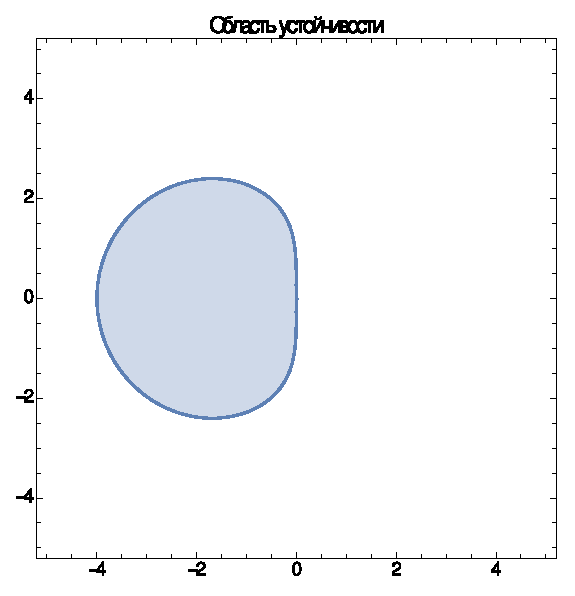
\includegraphics[width=.45\textwidth]{test_gr1.eps}\quad%
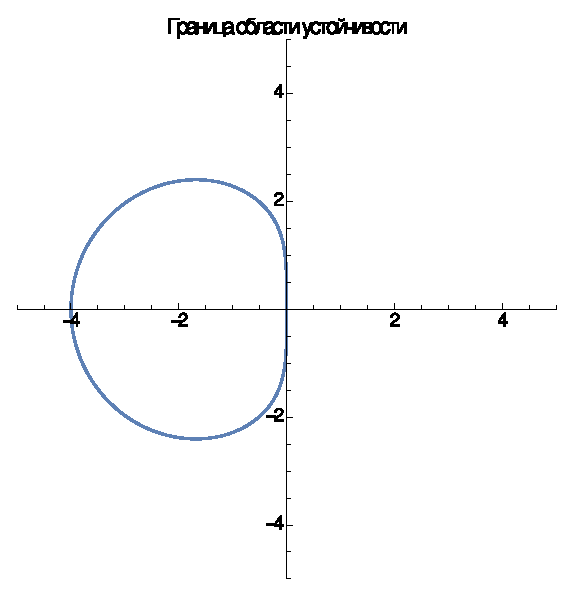
\includegraphics[width=.45\textwidth]{test_gr2.eps}
\caption{Область $|q_{1,2}(z)| < 1$ и ее граница $z(\phi)$} 
\end{figure}

Рассмотрим другой пример, на этот раз $A$-устойчивого метода ФДН2 (задача \textbf{T7})
\[
3 \vec u_{n+1} - 4 \vec u_n + \vec u_{n-1} = 2 \tau \vec G(t_{n+1}, \vec u_{n+1})
\]
Он характеризуется набором коэффициентов 
\[
a_2 = 3, \quad a_1 = -4, \quad a_0 = 1, \quad b_2 = 2, \quad b_1 = b_0 = 0
\]
Для него определяющая величина
\[
Q \operatorname{Re} z = 6 - 2 - 8 \cos \phi + 4 \cos^2 \phi = 4 (\cos \phi - 1)^2 \geqslant 0
\]
Чтобы показать $A$-устойчивость остается лишь проверить, что областью
устойчивости является внешность, а не внутренность кривой. Для этих целей обычно
удобно проверять $z = -\infty$ или $z = 0-\epsilon$.
Для ФДН-метода
\[
q_{1,2}(z) = \frac{2 \pm \sqrt{1 + 2z}}{3 - 2z}.
\]
Обе функции устойчивости при $z \rightarrow -\infty$ меньше единицы по модулю (так как стремятся к нулю), что завершает доказательство $A$-устойчивости.

\begin{figure}[ht!]
\centering
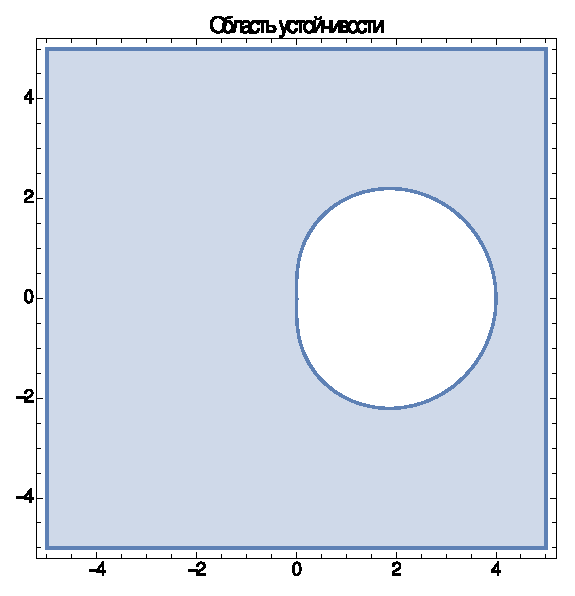
\includegraphics[width=.45\textwidth]{test2_gr1.eps}\quad%
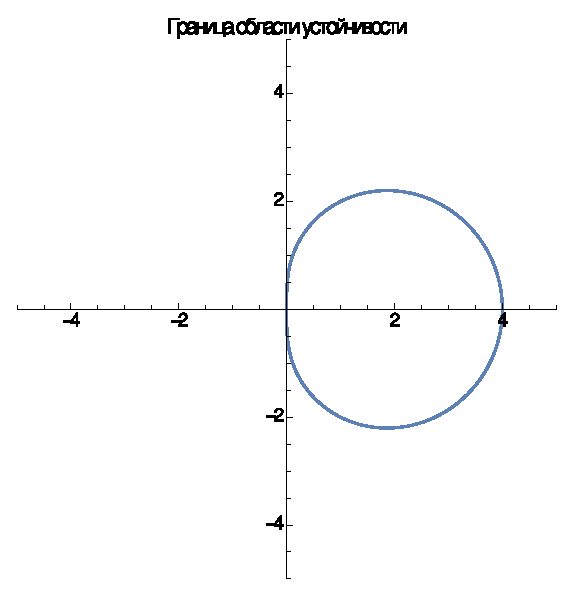
\includegraphics[width=.45\textwidth]{test2_gr2.eps}
\caption{Область $|q_{1,2}(z)| < 1$ и ее граница $z(\phi)$ для ФДН-метода}
\end{figure}

в) Поскольку $L$-устойчивым может быть только $A$-устойчивый метод, наш метод не $L$-устойчив.

Но ФДН метод, рассмотренный в предыдущем пункте является $L$-устойчивым, поскольку обе его функции устойчивости $q_{1,2}(z)$ стремятся по модулю при $z \rightarrow -\infty$ к нулю.

\end{document}
